% Options for packages loaded elsewhere
\PassOptionsToPackage{unicode}{hyperref}
\PassOptionsToPackage{hyphens}{url}
%
\documentclass[
]{article}
\usepackage{amsmath,amssymb}
\usepackage{lmodern}
\usepackage{iftex}
\ifPDFTeX
  \usepackage[T1]{fontenc}
  \usepackage[utf8]{inputenc}
  \usepackage{textcomp} % provide euro and other symbols
\else % if luatex or xetex
  \usepackage{unicode-math}
  \defaultfontfeatures{Scale=MatchLowercase}
  \defaultfontfeatures[\rmfamily]{Ligatures=TeX,Scale=1}
\fi
% Use upquote if available, for straight quotes in verbatim environments
\IfFileExists{upquote.sty}{\usepackage{upquote}}{}
\IfFileExists{microtype.sty}{% use microtype if available
  \usepackage[]{microtype}
  \UseMicrotypeSet[protrusion]{basicmath} % disable protrusion for tt fonts
}{}
\makeatletter
\@ifundefined{KOMAClassName}{% if non-KOMA class
  \IfFileExists{parskip.sty}{%
    \usepackage{parskip}
  }{% else
    \setlength{\parindent}{0pt}
    \setlength{\parskip}{6pt plus 2pt minus 1pt}}
}{% if KOMA class
  \KOMAoptions{parskip=half}}
\makeatother
\usepackage{xcolor}
\usepackage[margin=1in]{geometry}
\usepackage{color}
\usepackage{fancyvrb}
\newcommand{\VerbBar}{|}
\newcommand{\VERB}{\Verb[commandchars=\\\{\}]}
\DefineVerbatimEnvironment{Highlighting}{Verbatim}{commandchars=\\\{\}}
% Add ',fontsize=\small' for more characters per line
\usepackage{framed}
\definecolor{shadecolor}{RGB}{248,248,248}
\newenvironment{Shaded}{\begin{snugshade}}{\end{snugshade}}
\newcommand{\AlertTok}[1]{\textcolor[rgb]{0.94,0.16,0.16}{#1}}
\newcommand{\AnnotationTok}[1]{\textcolor[rgb]{0.56,0.35,0.01}{\textbf{\textit{#1}}}}
\newcommand{\AttributeTok}[1]{\textcolor[rgb]{0.77,0.63,0.00}{#1}}
\newcommand{\BaseNTok}[1]{\textcolor[rgb]{0.00,0.00,0.81}{#1}}
\newcommand{\BuiltInTok}[1]{#1}
\newcommand{\CharTok}[1]{\textcolor[rgb]{0.31,0.60,0.02}{#1}}
\newcommand{\CommentTok}[1]{\textcolor[rgb]{0.56,0.35,0.01}{\textit{#1}}}
\newcommand{\CommentVarTok}[1]{\textcolor[rgb]{0.56,0.35,0.01}{\textbf{\textit{#1}}}}
\newcommand{\ConstantTok}[1]{\textcolor[rgb]{0.00,0.00,0.00}{#1}}
\newcommand{\ControlFlowTok}[1]{\textcolor[rgb]{0.13,0.29,0.53}{\textbf{#1}}}
\newcommand{\DataTypeTok}[1]{\textcolor[rgb]{0.13,0.29,0.53}{#1}}
\newcommand{\DecValTok}[1]{\textcolor[rgb]{0.00,0.00,0.81}{#1}}
\newcommand{\DocumentationTok}[1]{\textcolor[rgb]{0.56,0.35,0.01}{\textbf{\textit{#1}}}}
\newcommand{\ErrorTok}[1]{\textcolor[rgb]{0.64,0.00,0.00}{\textbf{#1}}}
\newcommand{\ExtensionTok}[1]{#1}
\newcommand{\FloatTok}[1]{\textcolor[rgb]{0.00,0.00,0.81}{#1}}
\newcommand{\FunctionTok}[1]{\textcolor[rgb]{0.00,0.00,0.00}{#1}}
\newcommand{\ImportTok}[1]{#1}
\newcommand{\InformationTok}[1]{\textcolor[rgb]{0.56,0.35,0.01}{\textbf{\textit{#1}}}}
\newcommand{\KeywordTok}[1]{\textcolor[rgb]{0.13,0.29,0.53}{\textbf{#1}}}
\newcommand{\NormalTok}[1]{#1}
\newcommand{\OperatorTok}[1]{\textcolor[rgb]{0.81,0.36,0.00}{\textbf{#1}}}
\newcommand{\OtherTok}[1]{\textcolor[rgb]{0.56,0.35,0.01}{#1}}
\newcommand{\PreprocessorTok}[1]{\textcolor[rgb]{0.56,0.35,0.01}{\textit{#1}}}
\newcommand{\RegionMarkerTok}[1]{#1}
\newcommand{\SpecialCharTok}[1]{\textcolor[rgb]{0.00,0.00,0.00}{#1}}
\newcommand{\SpecialStringTok}[1]{\textcolor[rgb]{0.31,0.60,0.02}{#1}}
\newcommand{\StringTok}[1]{\textcolor[rgb]{0.31,0.60,0.02}{#1}}
\newcommand{\VariableTok}[1]{\textcolor[rgb]{0.00,0.00,0.00}{#1}}
\newcommand{\VerbatimStringTok}[1]{\textcolor[rgb]{0.31,0.60,0.02}{#1}}
\newcommand{\WarningTok}[1]{\textcolor[rgb]{0.56,0.35,0.01}{\textbf{\textit{#1}}}}
\usepackage{graphicx}
\makeatletter
\def\maxwidth{\ifdim\Gin@nat@width>\linewidth\linewidth\else\Gin@nat@width\fi}
\def\maxheight{\ifdim\Gin@nat@height>\textheight\textheight\else\Gin@nat@height\fi}
\makeatother
% Scale images if necessary, so that they will not overflow the page
% margins by default, and it is still possible to overwrite the defaults
% using explicit options in \includegraphics[width, height, ...]{}
\setkeys{Gin}{width=\maxwidth,height=\maxheight,keepaspectratio}
% Set default figure placement to htbp
\makeatletter
\def\fps@figure{htbp}
\makeatother
\setlength{\emergencystretch}{3em} % prevent overfull lines
\providecommand{\tightlist}{%
  \setlength{\itemsep}{0pt}\setlength{\parskip}{0pt}}
\setcounter{secnumdepth}{-\maxdimen} % remove section numbering
\ifLuaTeX
  \usepackage{selnolig}  % disable illegal ligatures
\fi
\IfFileExists{bookmark.sty}{\usepackage{bookmark}}{\usepackage{hyperref}}
\IfFileExists{xurl.sty}{\usepackage{xurl}}{} % add URL line breaks if available
\urlstyle{same} % disable monospaced font for URLs
\hypersetup{
  pdftitle={Data analysis for 4-methyl phenol from digestate experiments},
  pdfauthor={Sasha D. Hafner},
  hidelinks,
  pdfcreator={LaTeX via pandoc}}

\title{Data analysis for 4-methyl phenol from digestate experiments}
\author{Sasha D. Hafner}
\date{04 december, 2022}

\begin{document}
\maketitle

\hypertarget{plots}{%
\section{Plots}\label{plots}}

\begin{Shaded}
\begin{Highlighting}[]
\FunctionTok{ggplot}\NormalTok{(dat, }\FunctionTok{aes}\NormalTok{(time.end, fmp, }\AttributeTok{colour =}\NormalTok{ treatment, }\AttributeTok{group =} \FunctionTok{interaction}\NormalTok{(tunnel, treatment))) }\SpecialCharTok{+}
  \FunctionTok{geom\_line}\NormalTok{() }\SpecialCharTok{+}
  \FunctionTok{geom\_point}\NormalTok{() }\SpecialCharTok{+}
  \FunctionTok{facet\_wrap}\NormalTok{(}\SpecialCharTok{\textasciitilde{}}\NormalTok{ experiment)}
\end{Highlighting}
\end{Shaded}

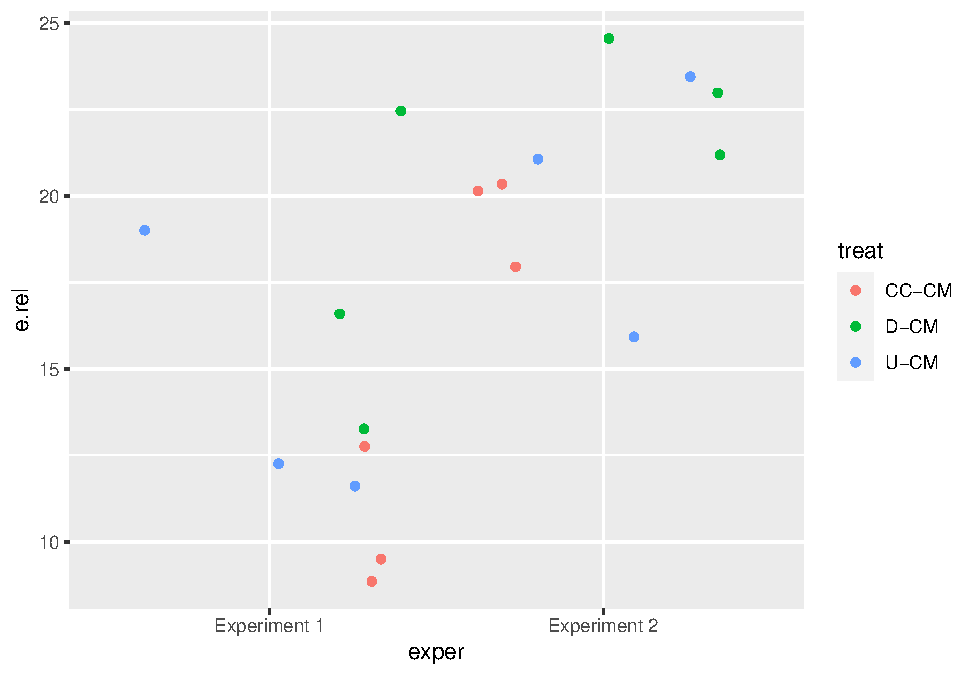
\includegraphics{C:/Users/au583430/OneDrive - Aarhus Universitet/Dokumenter/GitHub/Lemes-2022-digestate-NH3/output-stats/4mp_analysis_files/figure-latex/unnamed-chunk-1-1.pdf}

\hypertarget{stats}{%
\section{Stats}\label{stats}}

Set reference to untreatmented cattle manure.

Unit of analysis will be wind tunnel plot.

First fit model to each wind tunnel to get the ks.

Look at fit.

\begin{Shaded}
\begin{Highlighting}[]
\FunctionTok{ggplot}\NormalTok{(dat, }\FunctionTok{aes}\NormalTok{(time.end, fmp, }\AttributeTok{colour =}\NormalTok{ treatment, }\AttributeTok{group =} \FunctionTok{interaction}\NormalTok{(tunnel, treatment))) }\SpecialCharTok{+}
  \FunctionTok{geom\_line}\NormalTok{() }\SpecialCharTok{+}
  \FunctionTok{geom\_point}\NormalTok{() }\SpecialCharTok{+}
  \FunctionTok{geom\_line}\NormalTok{(}\FunctionTok{aes}\NormalTok{(time.end, fmp.calc), }\AttributeTok{lty =} \StringTok{\textquotesingle{}11\textquotesingle{}}\NormalTok{) }\SpecialCharTok{+}
  \FunctionTok{facet\_wrap}\NormalTok{(}\SpecialCharTok{\textasciitilde{}}\NormalTok{ experiment)}
\end{Highlighting}
\end{Shaded}

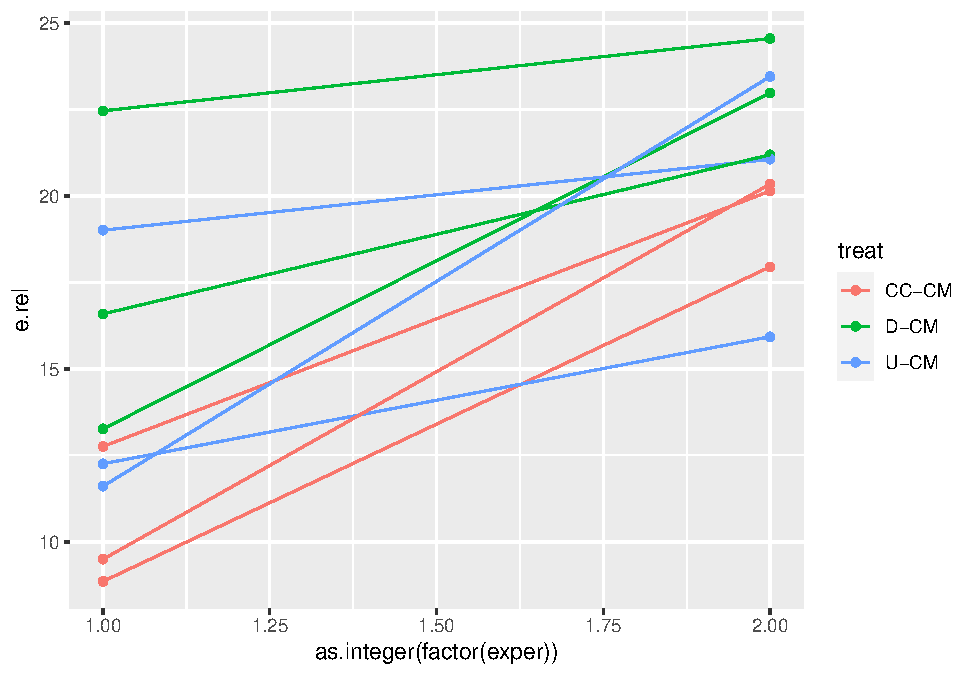
\includegraphics{C:/Users/au583430/OneDrive - Aarhus Universitet/Dokumenter/GitHub/Lemes-2022-digestate-NH3/output-stats/4mp_analysis_files/figure-latex/unnamed-chunk-2-1.pdf}

Take a look at km values.

\begin{Shaded}
\begin{Highlighting}[]
\FunctionTok{ggplot}\NormalTok{(lmods, }\FunctionTok{aes}\NormalTok{(experiment, km, }\AttributeTok{fill =}\NormalTok{ treatment)) }\SpecialCharTok{+}
  \FunctionTok{geom\_boxplot}\NormalTok{()}
\end{Highlighting}
\end{Shaded}

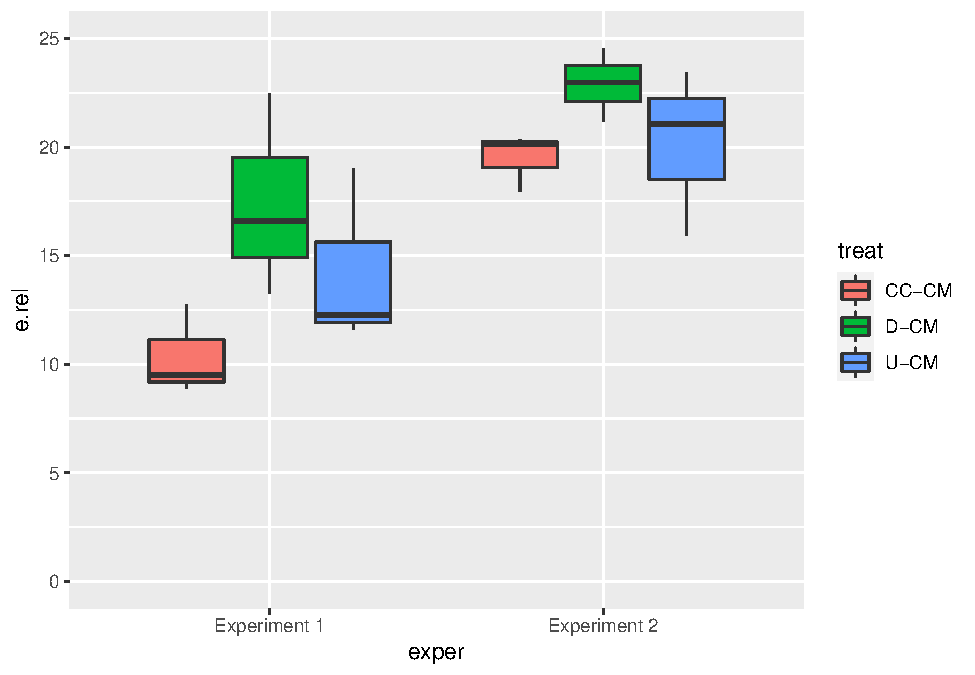
\includegraphics{C:/Users/au583430/OneDrive - Aarhus Universitet/Dokumenter/GitHub/Lemes-2022-digestate-NH3/output-stats/4mp_analysis_files/figure-latex/unnamed-chunk-3-1.pdf}

Now analysis.

\begin{Shaded}
\begin{Highlighting}[]
\NormalTok{modk1 }\OtherTok{\textless{}{-}} \FunctionTok{lm}\NormalTok{(km }\SpecialCharTok{\textasciitilde{}}\NormalTok{ treatment }\SpecialCharTok{*}\NormalTok{ experiment, }\AttributeTok{data =}\NormalTok{ lmods)}
\FunctionTok{summary.aov}\NormalTok{(modk1)}
\end{Highlighting}
\end{Shaded}

\begin{verbatim}
##                      Df Sum Sq Mean Sq F value   Pr(>F)    
## treatment             2  42.19   21.10   72.25 2.03e-07 ***
## experiment            1 171.80  171.80  588.38 1.45e-11 ***
## treatment:experiment  2  11.44    5.72   19.59 0.000166 ***
## Residuals            12   3.50    0.29                     
## ---
## Signif. codes:  0 '***' 0.001 '**' 0.01 '*' 0.05 '.' 0.1 ' ' 1
\end{verbatim}

\begin{Shaded}
\begin{Highlighting}[]
\FunctionTok{summary}\NormalTok{(modk1)}
\end{Highlighting}
\end{Shaded}

\begin{verbatim}
## 
## Call:
## lm(formula = km ~ treatment * experiment, data = lmods)
## 
## Residuals:
##      Min       1Q   Median       3Q      Max 
## -0.84027 -0.22806  0.01571  0.26198  1.15075 
## 
## Coefficients:
##                                         Estimate Std. Error t value Pr(>|t|)    
## (Intercept)                              12.1068     0.3120  38.807 5.52e-14 ***
## treatmentD-CM                            -1.6571     0.4412  -3.756  0.00274 ** 
## treatmentD-CM-CC                         -5.5330     0.4412 -12.541 2.95e-08 ***
## experimentExperiment 2                   -7.6197     0.4412 -17.271 7.68e-10 ***
## treatmentD-CM:experimentExperiment 2      0.6594     0.6239   1.057  0.31141    
## treatmentD-CM-CC:experimentExperiment 2   3.6635     0.6239   5.872 7.58e-05 ***
## ---
## Signif. codes:  0 '***' 0.001 '**' 0.01 '*' 0.05 '.' 0.1 ' ' 1
## 
## Residual standard error: 0.5404 on 12 degrees of freedom
## Multiple R-squared:  0.9847, Adjusted R-squared:  0.9783 
## F-statistic: 154.4 on 5 and 12 DF,  p-value: 1.848e-10
\end{verbatim}

Interactions complicated. Let's look by experiment. First experiment 1.

\begin{Shaded}
\begin{Highlighting}[]
\NormalTok{modexp1 }\OtherTok{\textless{}{-}} \FunctionTok{aov}\NormalTok{(km }\SpecialCharTok{\textasciitilde{}}\NormalTok{ treatment, }\AttributeTok{data =}\NormalTok{ lmods, }\AttributeTok{subset =}\NormalTok{ experiment }\SpecialCharTok{==} \StringTok{\textquotesingle{}Experiment 1\textquotesingle{}}\NormalTok{)}
\FunctionTok{summary}\NormalTok{(modexp1)}
\end{Highlighting}
\end{Shaded}

\begin{verbatim}
##             Df Sum Sq Mean Sq F value   Pr(>F)    
## treatment    2  48.38  24.191   59.98 0.000108 ***
## Residuals    6   2.42   0.403                     
## ---
## Signif. codes:  0 '***' 0.001 '**' 0.01 '*' 0.05 '.' 0.1 ' ' 1
\end{verbatim}

\begin{Shaded}
\begin{Highlighting}[]
\FunctionTok{summary.lm}\NormalTok{(modexp1)}
\end{Highlighting}
\end{Shaded}

\begin{verbatim}
## 
## Call:
## aov(formula = km ~ treatment, data = lmods, subset = experiment == 
##     "Experiment 1")
## 
## Residuals:
##      Min       1Q   Median       3Q      Max 
## -0.84027 -0.31048  0.01001  0.20598  1.15075 
## 
## Coefficients:
##                  Estimate Std. Error t value Pr(>|t|)    
## (Intercept)       12.1068     0.3667  33.019 5.13e-08 ***
## treatmentD-CM     -1.6571     0.5185  -3.196   0.0187 *  
## treatmentD-CM-CC  -5.5330     0.5185 -10.670 4.00e-05 ***
## ---
## Signif. codes:  0 '***' 0.001 '**' 0.01 '*' 0.05 '.' 0.1 ' ' 1
## 
## Residual standard error: 0.6351 on 6 degrees of freedom
## Multiple R-squared:  0.9524, Adjusted R-squared:  0.9365 
## F-statistic: 59.98 on 2 and 6 DF,  p-value: 0.0001081
\end{verbatim}

\begin{Shaded}
\begin{Highlighting}[]
\FunctionTok{coef}\NormalTok{(modexp1)}
\end{Highlighting}
\end{Shaded}

\begin{verbatim}
##      (Intercept)    treatmentD-CM treatmentD-CM-CC 
##        12.106822        -1.657076        -5.532987
\end{verbatim}

\begin{Shaded}
\begin{Highlighting}[]
\FunctionTok{confint}\NormalTok{(modexp1)}
\end{Highlighting}
\end{Shaded}

\begin{verbatim}
##                      2.5 %     97.5 %
## (Intercept)      11.209638 13.0040051
## treatmentD-CM    -2.925885 -0.3882667
## treatmentD-CM-CC -6.801796 -4.2641781
\end{verbatim}

\begin{Shaded}
\begin{Highlighting}[]
\FunctionTok{model.tables}\NormalTok{(modexp1, }\AttributeTok{type =} \StringTok{\textquotesingle{}means\textquotesingle{}}\NormalTok{)}
\end{Highlighting}
\end{Shaded}

\begin{verbatim}
## Tables of means
## Grand mean
##          
## 9.710134 
## 
##  treatment 
## treatment
##    U-CM    D-CM D-CM-CC 
##  12.107  10.450   6.574
\end{verbatim}

\textbf{Use this model in paper.} Both D-CM and CC-CM have lower k than
reference in experiment 1.

Experiment 2 next.

\begin{Shaded}
\begin{Highlighting}[]
\NormalTok{modexp2 }\OtherTok{\textless{}{-}} \FunctionTok{aov}\NormalTok{(km }\SpecialCharTok{\textasciitilde{}}\NormalTok{ treatment, }\AttributeTok{data =}\NormalTok{ lmods, }\AttributeTok{subset =}\NormalTok{ experiment }\SpecialCharTok{==} \StringTok{\textquotesingle{}Experiment 2\textquotesingle{}}\NormalTok{)}
\FunctionTok{summary}\NormalTok{(modexp2)}
\end{Highlighting}
\end{Shaded}

\begin{verbatim}
##             Df Sum Sq Mean Sq F value  Pr(>F)   
## treatment    2  5.250  2.6252   14.53 0.00501 **
## Residuals    6  1.084  0.1806                   
## ---
## Signif. codes:  0 '***' 0.001 '**' 0.01 '*' 0.05 '.' 0.1 ' ' 1
\end{verbatim}

\begin{Shaded}
\begin{Highlighting}[]
\FunctionTok{summary.lm}\NormalTok{(modexp2)}
\end{Highlighting}
\end{Shaded}

\begin{verbatim}
## 
## Call:
## aov(formula = km ~ treatment, data = lmods, subset = experiment == 
##     "Experiment 2")
## 
## Residuals:
##     Min      1Q  Median      3Q     Max 
## -0.7572 -0.2184  0.0214  0.2832  0.3935 
## 
## Coefficients:
##                  Estimate Std. Error t value Pr(>|t|)    
## (Intercept)        4.4871     0.2454  18.286 1.72e-06 ***
## treatmentD-CM     -0.9977     0.3470  -2.875  0.02825 *  
## treatmentD-CM-CC  -1.8695     0.3470  -5.387  0.00168 ** 
## ---
## Signif. codes:  0 '***' 0.001 '**' 0.01 '*' 0.05 '.' 0.1 ' ' 1
## 
## Residual standard error: 0.425 on 6 degrees of freedom
## Multiple R-squared:  0.8289, Adjusted R-squared:  0.7718 
## F-statistic: 14.53 on 2 and 6 DF,  p-value: 0.00501
\end{verbatim}

\begin{Shaded}
\begin{Highlighting}[]
\FunctionTok{coef}\NormalTok{(modexp2)}
\end{Highlighting}
\end{Shaded}

\begin{verbatim}
##      (Intercept)    treatmentD-CM treatmentD-CM-CC 
##        4.4870880       -0.9976791       -1.8694707
\end{verbatim}

\begin{Shaded}
\begin{Highlighting}[]
\FunctionTok{confint}\NormalTok{(modexp2)}
\end{Highlighting}
\end{Shaded}

\begin{verbatim}
##                      2.5 %     97.5 %
## (Intercept)       3.886645  5.0875310
## treatmentD-CM    -1.846834 -0.1485246
## treatmentD-CM-CC -2.718625 -1.0203161
\end{verbatim}

\begin{Shaded}
\begin{Highlighting}[]
\FunctionTok{model.tables}\NormalTok{(modexp2, }\AttributeTok{type =} \StringTok{\textquotesingle{}means\textquotesingle{}}\NormalTok{)}
\end{Highlighting}
\end{Shaded}

\begin{verbatim}
## Tables of means
## Grand mean
##          
## 3.531371 
## 
##  treatment 
## treatment
##    U-CM    D-CM D-CM-CC 
##   4.487   3.489   2.618
\end{verbatim}

Both D-CM and CC-CM have lower k than reference in experiment 2.
\textbf{Use this model in paper for experiment 2.}

Diagnostic plots.

\begin{Shaded}
\begin{Highlighting}[]
\FunctionTok{plot}\NormalTok{(modexp1, }\AttributeTok{ask =} \ConstantTok{FALSE}\NormalTok{)}
\end{Highlighting}
\end{Shaded}

\includegraphics{C:/Users/au583430/OneDrive - Aarhus Universitet/Dokumenter/GitHub/Lemes-2022-digestate-NH3/output-stats/4mp_analysis_files/figure-latex/unnamed-chunk-7-1.pdf}
\includegraphics{C:/Users/au583430/OneDrive - Aarhus Universitet/Dokumenter/GitHub/Lemes-2022-digestate-NH3/output-stats/4mp_analysis_files/figure-latex/unnamed-chunk-7-2.pdf}
\includegraphics{C:/Users/au583430/OneDrive - Aarhus Universitet/Dokumenter/GitHub/Lemes-2022-digestate-NH3/output-stats/4mp_analysis_files/figure-latex/unnamed-chunk-7-3.pdf}
\includegraphics{C:/Users/au583430/OneDrive - Aarhus Universitet/Dokumenter/GitHub/Lemes-2022-digestate-NH3/output-stats/4mp_analysis_files/figure-latex/unnamed-chunk-7-4.pdf}

\begin{Shaded}
\begin{Highlighting}[]
\FunctionTok{plot}\NormalTok{(modexp2, }\AttributeTok{ask =} \ConstantTok{FALSE}\NormalTok{)}
\end{Highlighting}
\end{Shaded}

\includegraphics{C:/Users/au583430/OneDrive - Aarhus Universitet/Dokumenter/GitHub/Lemes-2022-digestate-NH3/output-stats/4mp_analysis_files/figure-latex/unnamed-chunk-8-1.pdf}
\includegraphics{C:/Users/au583430/OneDrive - Aarhus Universitet/Dokumenter/GitHub/Lemes-2022-digestate-NH3/output-stats/4mp_analysis_files/figure-latex/unnamed-chunk-8-2.pdf}
\includegraphics{C:/Users/au583430/OneDrive - Aarhus Universitet/Dokumenter/GitHub/Lemes-2022-digestate-NH3/output-stats/4mp_analysis_files/figure-latex/unnamed-chunk-8-3.pdf}
\includegraphics{C:/Users/au583430/OneDrive - Aarhus Universitet/Dokumenter/GitHub/Lemes-2022-digestate-NH3/output-stats/4mp_analysis_files/figure-latex/unnamed-chunk-8-4.pdf}

Not terrible.

Now initial flux.

\begin{Shaded}
\begin{Highlighting}[]
\NormalTok{modf1 }\OtherTok{\textless{}{-}} \FunctionTok{aov}\NormalTok{(}\FunctionTok{log10}\NormalTok{(fmp) }\SpecialCharTok{\textasciitilde{}}\NormalTok{ experiment }\SpecialCharTok{*}\NormalTok{ treatment, }\AttributeTok{data =}\NormalTok{ d1)}
\FunctionTok{summary}\NormalTok{(modf1)}
\end{Highlighting}
\end{Shaded}

\begin{verbatim}
##                      Df Sum Sq Mean Sq F value   Pr(>F)    
## experiment            1 1.3079  1.3079 395.964 1.48e-10 ***
## treatment             2 0.4860  0.2430  73.573 1.84e-07 ***
## experiment:treatment  2 0.0055  0.0027   0.826    0.461    
## Residuals            12 0.0396  0.0033                     
## ---
## Signif. codes:  0 '***' 0.001 '**' 0.01 '*' 0.05 '.' 0.1 ' ' 1
\end{verbatim}

\begin{Shaded}
\begin{Highlighting}[]
\FunctionTok{summary.lm}\NormalTok{(modf1)}
\end{Highlighting}
\end{Shaded}

\begin{verbatim}
## 
## Call:
## aov(formula = log10(fmp) ~ experiment * treatment, data = d1)
## 
## Residuals:
##       Min        1Q    Median        3Q       Max 
## -0.085332 -0.023807 -0.002667  0.031886  0.085321 
## 
## Coefficients:
##                                         Estimate Std. Error t value Pr(>|t|)    
## (Intercept)                              0.69339    0.03318  20.897 8.35e-11 ***
## experimentExperiment 2                   0.58785    0.04693  12.527 2.99e-08 ***
## treatmentD-CM                           -0.02403    0.04693  -0.512    0.618    
## treatmentD-CM-CC                        -0.34251    0.04693  -7.299 9.49e-06 ***
## experimentExperiment 2:treatmentD-CM    -0.07923    0.06636  -1.194    0.256    
## experimentExperiment 2:treatmentD-CM-CC -0.06699    0.06636  -1.010    0.333    
## ---
## Signif. codes:  0 '***' 0.001 '**' 0.01 '*' 0.05 '.' 0.1 ' ' 1
## 
## Residual standard error: 0.05747 on 12 degrees of freedom
## Multiple R-squared:  0.9784, Adjusted R-squared:  0.9695 
## F-statistic:   109 on 5 and 12 DF,  p-value: 1.429e-09
\end{verbatim}

\begin{Shaded}
\begin{Highlighting}[]
\DecValTok{100} \SpecialCharTok{*}\NormalTok{ (}\DecValTok{1} \SpecialCharTok{{-}} \DecValTok{10}\SpecialCharTok{\^{}}\FunctionTok{coef}\NormalTok{(modf1))}
\end{Highlighting}
\end{Shaded}

\begin{verbatim}
##                             (Intercept)                  experimentExperiment 2                           treatmentD-CM 
##                             -393.613664                             -287.122291                                5.382188 
##                        treatmentD-CM-CC    experimentExperiment 2:treatmentD-CM experimentExperiment 2:treatmentD-CM-CC 
##                               54.554974                               16.675567                               14.295225
\end{verbatim}

\begin{Shaded}
\begin{Highlighting}[]
\DecValTok{100} \SpecialCharTok{*}\NormalTok{ (}\DecValTok{1} \SpecialCharTok{{-}} \DecValTok{10}\SpecialCharTok{\^{}}\FunctionTok{confint}\NormalTok{(modf1))}
\end{Highlighting}
\end{Shaded}

\begin{verbatim}
##                                              2.5 %     97.5 %
## (Intercept)                             -317.91834 -483.01929
## experimentExperiment 2                  -205.91907 -389.88011
## treatmentD-CM                             25.22933  -19.73318
## treatmentD-CM-CC                          64.08758   42.49204
## experimentExperiment 2:treatmentD-CM      40.27160  -16.24221
## experimentExperiment 2:treatmentD-CM-CC   38.56533  -19.56292
\end{verbatim}

\end{document}
